\chapter{A Prototype PKG Tool} \label{ch:prototype}
% hm.. kannst du erläutern, wie man neue Nodes anlegt und editiert? Passiert das in Markdown? Kannst du da noch ein paar Screenshots spendieren? Welches Backend hast du drunter? Welches Storage Format? Hast du Usability Tests gemacht? Benutzt jemand das Tool außer dir? Welcher Tech-Stack? Welche Grundarchitektur hat die App? Welchen Code-Umfang? Hast du automatisierte Tests? Kann man das knallige Farbschema ändern? Würde mir auch eine stark reduziertere Ansicht wünschen, vielleicht eher tabellarisch, ohne diese gelabelten Pfeile, oder eher Paragraphen-Like, mehr wie Text, oder halt bei Notion - sieht aus wie Text, isses aber nicht. Welche Schnittstellen hast du - kann man damit RDFs von draußen importieren, oder exportieren? Und das wichtigste.. wo ist das Suchen-Eingabefeld? Wie sieht die Seite mobil aus?

While many challenges of PKGs can be addressed with the data model and architecture, the User Experience (UX) aspect needs to be considered separately. Semantic web technology is hard to understand even for Computer Scientists, as even the W3C acknowledges \cite{EasierRDF}. Expecting non-technical people to grasp all the concepts semantic web standards rely on is unrealistic. For personal use by non-technical people, these concepts need to be abstracted away with a self-explanatory User Interface (UI) aided by Tutorials. 

In this chapter, we present a prototype that aims to be user-friendly and not rely on previous knowledge of semantic web technologies \cite{missingCitation}.

\section{Tech-Stack}

The Prototype is implemented as a Web Application using HTML, CSS, TypeScript and the Frameworks TailwindCSS and Svelte \cite{missingCitation}. 

The RDF Data is stored in memory by using our implementation of the RDFJS specification called RDFun \cite{rdfjs}. RDFJS is a specification for working with RDF in JavaScript. A host of Libraries exist that provide functionality for RDF graph datasets that are compliant with RDFJS. We used libraries for fetching and querying external RDF data \cite{missingCitation} [rdfetch, comunica].

\section{Usability Considerations}

The prototype is implemented as a single page web app. This enables a frictionless setup without needing to download or configure a client.

No knowledge of semantic web technologies is necessary to use the app, even though it is based on the RDF data model.

\section{The User Interface} 

\begin{figure}[H]
    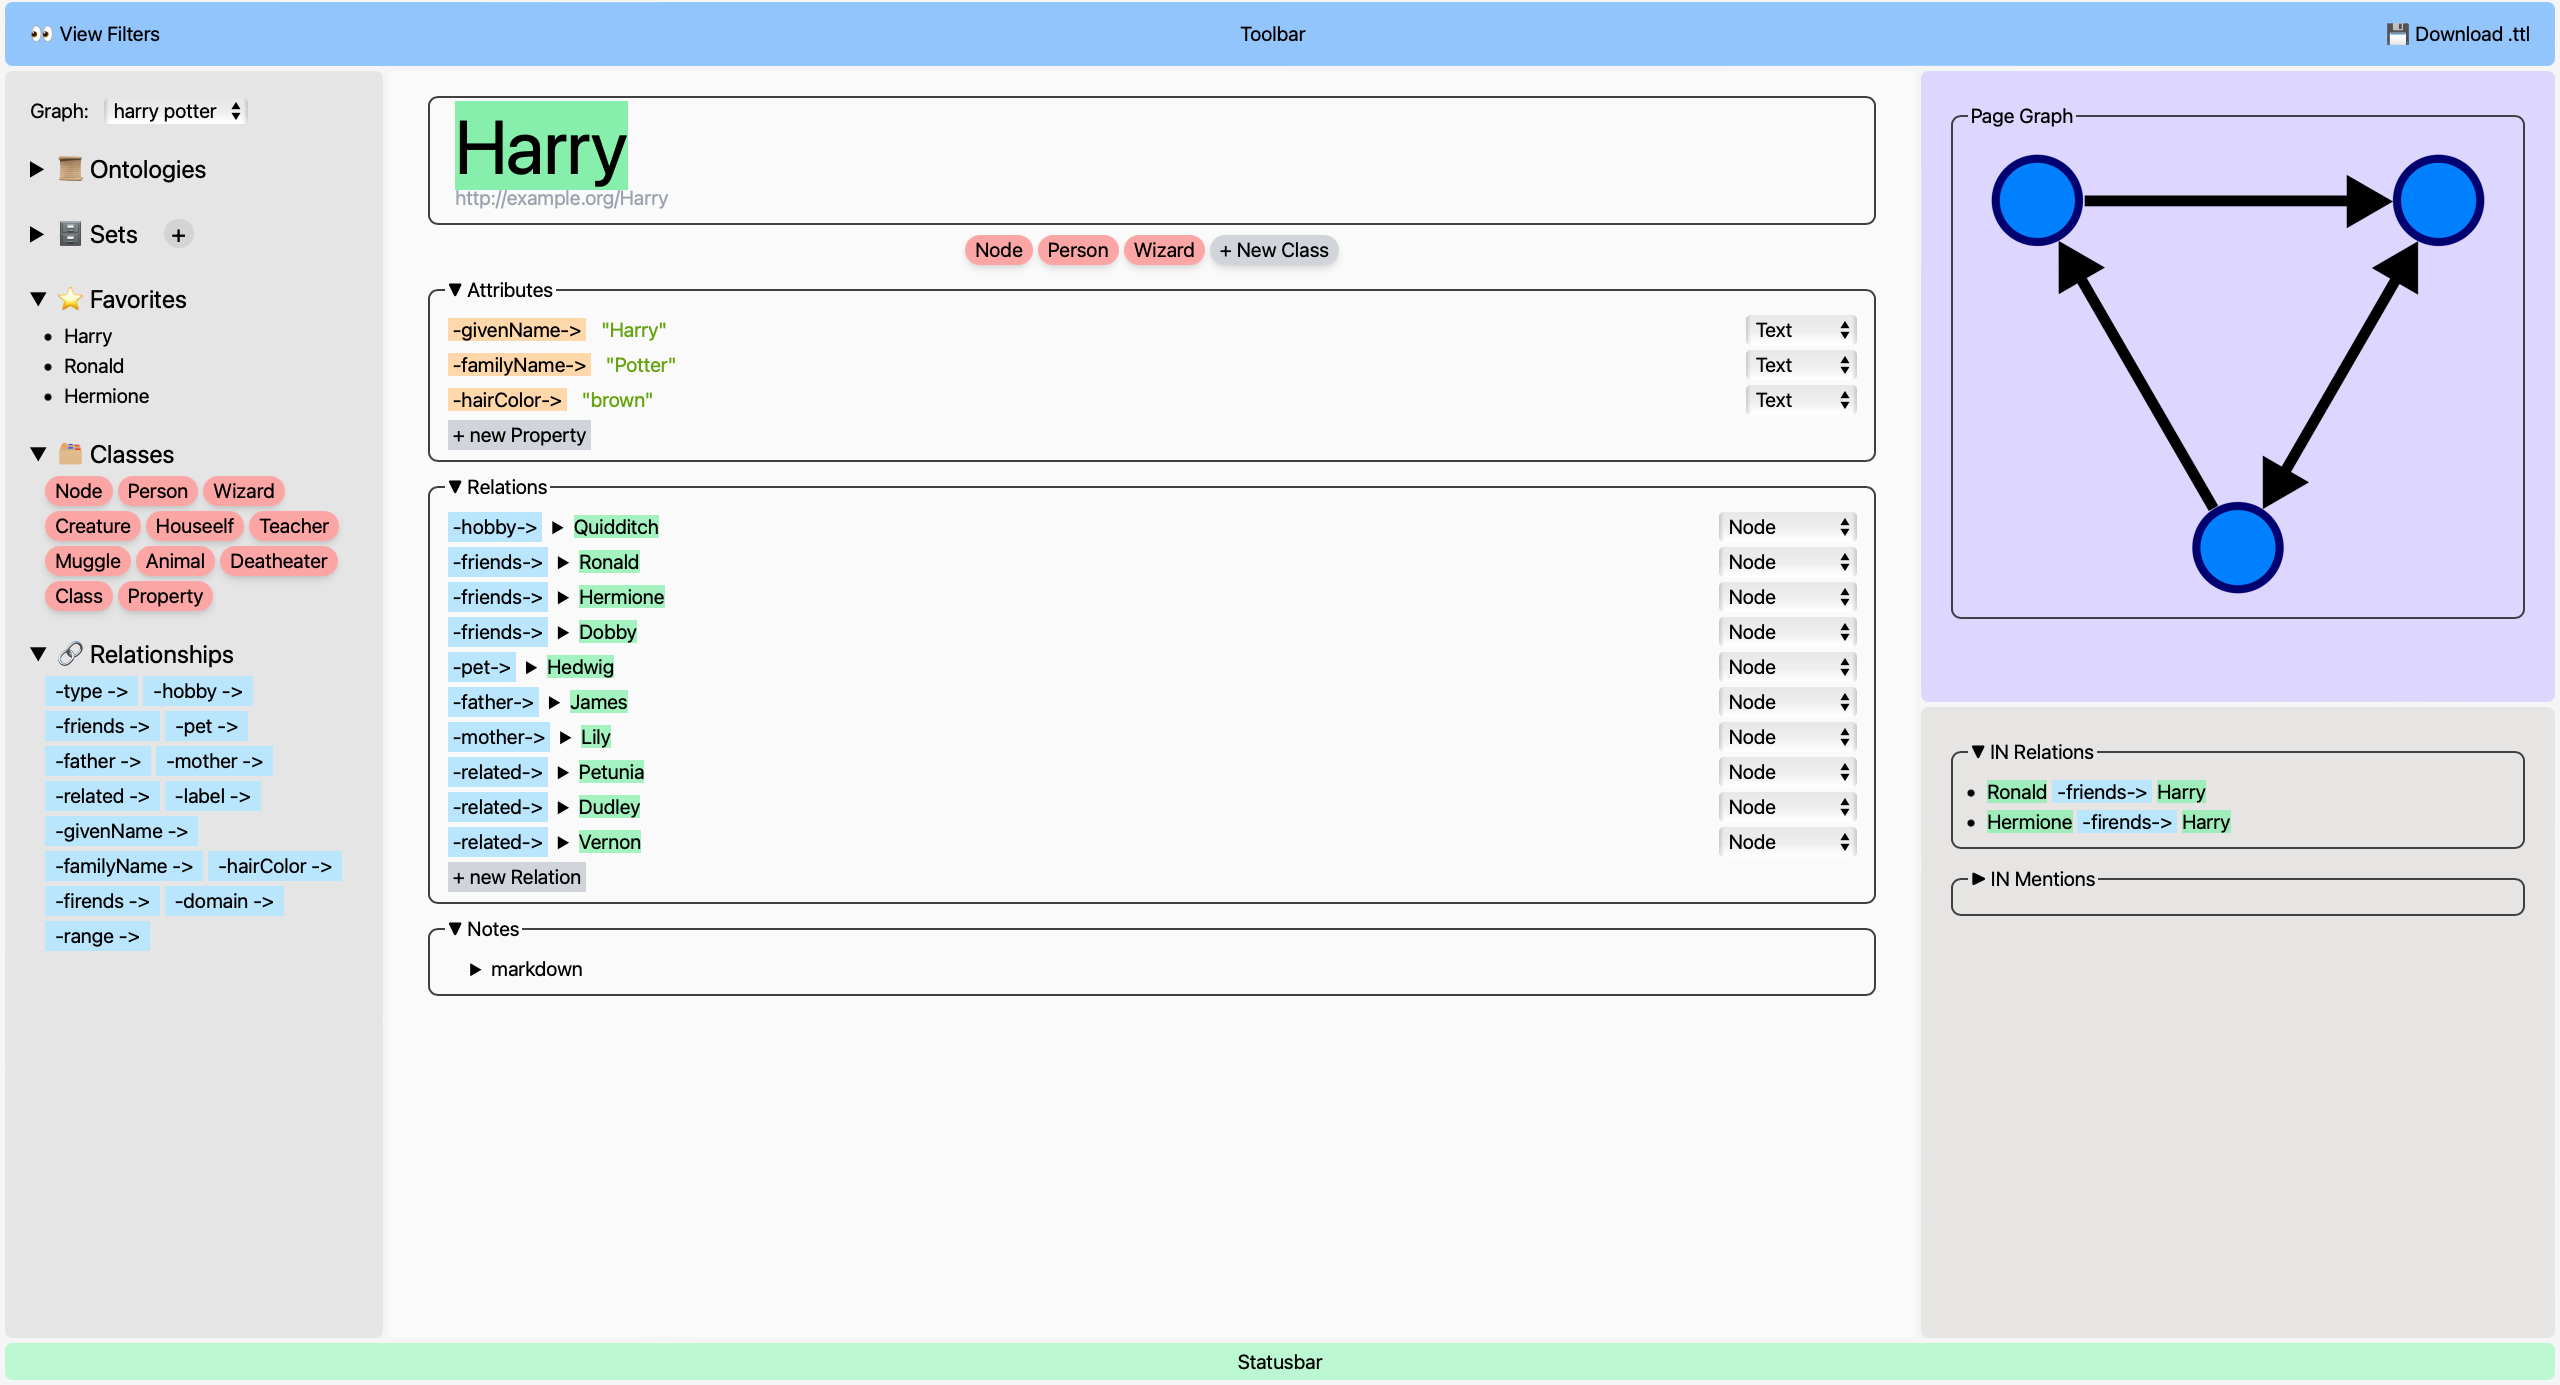
\includegraphics[width=\textwidth]{nink}
\end{figure}

Figure 7.1 shows a screenshot of the UI. It is divided into several Sections, some of them similar to sections found in Apps people frequently use, like note-taking apps, Wikipedia or email clients. From top left to bottom right:
\begin{description}
    \item[Toolbar] The Toolbar is similar to the ones found in modern browsers. It displays open Nodes in Tabs with the IRI appearing as the Title for the Tab. In the outermost corners are shortcuts for accessing prominent functionality.
    \item[Sidebar] The Sidebar serves as navigation and orientation. Users can navigate to Classes, Relationships and their favorite Nodes in the PKG. There are also overviews of used Schema and Sets / Views.
    \item[Editor] The Editor renders all the relevant Information about the currently active Node. The User can toggle which Information is relevant to him and navigate to related Nodes. He can also create, update and delete related Entities and Text.
    \item[Graph panel] The Graph Panel serves as an overview of the context of the current and associated Nodes in visualized form. This provides further orientation and a spatial sense of connectedness in the PKG.
    \item[Relation panel] The Relation Panel shows inferred relations and mentions. (Meaning arcs from other nodes to the current node.
\end{description}

The label and classes of the current node are placed in special positions and hidden from the Relations. The label is prominently displayed as the title, reminiscent of most Text Processors. Classes are presented right below it, similar to tags or categorys in other Applications. This is done to build on the familiarity with similar UIs the User might have interacted with.
    
Notice how Classes, Properties, Entities and Literals are all visually distinguished in the UI, highlighting their different nature and providing easy navigation of the content.

The Semantic Markdown is displayed in a outliner UI, as though it was a hierarchical attachment to the current Node. The structured semantics in it are displayed on the relevant Nodes in an opaque fashion, to hightlight the fact that they are not manifested in the data layer, but rather inferred from Notes. A button enables the user to transform them into explicit statements from the note layer into the data layer. Similar functionality is present for integrating external structured Data (like wikidata, dbpedia, etc.)

\section{Functionality}

The following is an overview of Features and Functionalities of the Prototype.

All of this functionality manipulates the Dataset as outlined in Chapter [Data Model], by creating, updating or deleting RDF triples.
\begin{description}
    \item[Create Node] Pressing the button labeled “+ New Node” in the botton left corner or using the keyboard shortcut “ctrl + n” creates a new Node in the Graph. The User is automatically navigated to the new Node and can edit the Title / Label.
    \item[Attach Class] A new Class can be attached to the current Node by clicking the “+ add Class” button right below the Title / Label.
    \item[Attach Attribute / Relationship] A RDF Triple with the Current Node in subject position can be created by pressing the “+ add Attribute / Relation” Button at the bottom of the respective Sections. This prompts the user to enter a label for the predicate (Relationship) and Object (Target Entity / Literal) of the triple.
    \item[Write Semantic Markdown] In the Notes Section, Semantic Markdown can be edited in an Outliner Text Processor Interface (This feature is not fully implemented yet).
    \item[Switch RDF Graph Dataset] The user can select the RDF Dataset in the “Graph” labeled select input in the Sidebar, to switch between Graph Datasets.
    \item[Import RDF Graphs from URL] The user can import RDF Data from external Sources, by selecting “+ import from URL” from the “Graph” labeled select input in the Sidebar.
\end{description}

